\chapter{Theory of the Drift-Wave Instability at Arbitrary Collisionality}
\label{ch:dwi}

Drift-waves (DW) are low-frequency modes that arise in a magnetized plasma when a finite pressure gradient is present, and are driven unstable when electron adiabaticity is broken, such as in the presence of finite resistivity, electron inertia or wave-particle resonances.
%
Due to the ubiquitous presence of pressure gradients and adiabaticity-breaking mechanisms in plasmas, the DW instability plays a role in many plasma systems \citep{Goldston1995}.
%
Indeed, DW are known to regulate plasma transport across the magnetic field in laboratory plasmas \citep{Horton1999,Scott2002,Burin2005,Poli2008,Schaffner2012,Mosetto2013}, and are also thought to be relevant for the understanding of fundamental transport processes occurring in active galactic nuclei \citep{Saleem2003}, dense astrophysical bodies \citep{Wu2008}, the Earth's magnetosphere \citep{Shukla1980}, and dusty plasmas \citep{Salimullah2009}.
%
In addition, the understanding of DW is crucial since the physics underlying a number of important plasmas instabilities, such as the electron- and ion-temperature gradient modes, resistive modes, and ballooning modes \citep{Stix1992}, relies on the same mechanisms at play in DW.

Although DW are the subject of a large number of previous studies, the effect of collisionality on the linear properties of these modes remains insufficiently understood. 
%
This is particularly worrisome since collisionality has been found to have both stabilizing \citep{Stix1992} and destabilizing effects \citep{White2014} on DW.
%
Previous studies on the DW instability at finite collisionality have usually relied on simplified collision operators \citep{Angus2012}, or on fluid models such as the Hasegawa-Wakatani \citep{Hasegawa1983} or the drift-reduced Braginskii model \citep{Ricci2012a}, which assume that the electron and ion collision frequencies are high enough so that the particle mean free path stays small when compared with the mode parallel wavelength, $k_\parallel \lambda_{mfp} \ll 1$.

%
In the present chapter, as a second investigation of the model described in \cref{ch:dk}, we overcome this long-standing issue and provide an efficient framework, which can be easily extended to a large number of instabilities in magnetized plasmas, to properly study the effect of collisionality in DW at arbitrary mean free path.
%
Here, we focus on the case where the DW driving mechanism is provided by the density gradient, usually referred to as the universal instability \citep{Landreman2015}, in a shearless slab geometry.
%
For simplicity, we consider the case where $B$ is uniform.
%
The DW growth rate that we evaluate matches both the collisionless and fluid regimes at low and high collision frequencies, respectively, and shows important deviations from the collisional limit already at $k_\parallel \lambda_{mfp} \sim 0.1$.
%
Furthermore, at low-to-intermediate collisionality values, the regime of interest for future tokamak devices such as ITER \citep{Aymar2002}, we show the need to retain the full Coulomb collision operator.
%
Indeed, the DW growth rate deviates by factors of order unity from fluid and kinetic models based on approximate collision operators such as the Lenard-Bernstein \citep{Lenard1958} and the Dougherty \citep{Dougherty1964} operators.
%
These operators, by being implemented in a number of advanced kinetic codes, are used in recent studies of DW-like turbulence, both in the core \citep{Hatch2013,Nakata2016,Grandgirard2016,Mandell2018} and at edge \citep{Shi2017,Pan2018} regions of tokamak devices.
%
Since quasi-linear transport models estimate the turbulence drive by evaluating the linear instability growth rate \citep{Chen2000,Bourdelle2015}, quantitative differences in the growth rate  have a large impact on the prediction of the level of transport, in particular by affecting the threshold for $\mathbf E \times \mathbf B$ shear flow stabilization.
%
Similarly, the linear growth rate, together with the gradient removal hypothesis \citep{Ricci2013}, is used to predict the SOL width, a parameter crucial to the overall performance of present and future tokamak devices such as ITER \citep{Halpern2013}.
%
Therefore, our results can impact ITER operation and the design of future fusion devices.

%
As for the EPW, in addition to the instability growth rate, the framework we propose allows the evaluation of the spectrum of the linear eigenmodes.
%
The spectrum of DW collisional eigenmodes, contrary to the collisionless case, is composed of a discrete set of roots, as first shown in \citep{Ng1999}.
%
Deviations between the results based on the Coulomb and both the Lenard-Bernstein and Dougherty collision operators are particularly evident.
%
The clear differences question our current understanding of plasma turbulence.
%
In fact, several DW turbulence studies have shown that subdominant and stable modes can be nonlinearly excited to finite amplitude \citep{Terry2006,Hatch2011,Hatch2011a,Pueschel2016} and have a major role in nonlinear energy dissipation and turbulence saturation, affecting structure formation, as well as heat and particle transport.
%
The computation of such modes relies on the correct evaluation of the eigenmode spectrum. 
%
{As we show, this displays large changes between the Coulomb and approximate collision operators}.

This chapter is organized as follows.
%
In \cref{sec:dwmechanism}, the basic mechanism behind the dynamics of DW is described.
%
\cref{sec:momhierarchymodeldw} derives the moment-hierarchy formalism at arbitrary collisionality used to study the DW instability.
%
In \cref{sec:dwnumericalresults}, the numerical results are presented.
%
The conclusions follow in \cref{sec:dwconclusion}.
%
We note that the results described in the present chapter have been published in \citep{Jorge2018}.

\section{Fundamental Mechanisms Determining the Drift-Wave Dynamics}
\label{sec:dwmechanism}

We consider a magnetized plasma in a straight and uniform magnetic field $\mathbf B$ along the $z$ direction.
%
Only electrostatic perturbations are studied, such that $\mathbf B = B \mathbf e_z$ with $B$ constant and $(\mathbf e_x, \mathbf e_y, \mathbf e_z)$ the Cartesian unit vectors.
%
In addition, we focus on scales $L$ larger than the Debye length $\lambda_D=\sqrt{T_0/(4\pi n_0 e^2)}\ll L$, so that the plasma can be considered to be quasineutral, i.e., 
%
\begin{equation}
    n_e \simeq n_i \simeq n.
\end{equation}
%
For the ion species, we consider the ion continuity equation
%
\begin{equation}
    \frac{\partial n}{\partial t}+\nabla \cdot( n \mathbf u_i) =0,
\label{eq:dw1}
\end{equation}
%
with $\mathbf u_i$ the ion fluid velocity given, in the cold ion limit, by the momentum equation
%
\begin{equation}
    m_i \frac{d \mathbf u_i}{dt}=-e \nabla \phi + e \mathbf u_i \times \mathbf B.
\label{eq:dw2}
\end{equation}
%
Solving \cref{eq:dw2} for the perpendicular ion velocity $\mathbf u_{\perp i}=( \mathbf b \times \mathbf u_i)\times \mathbf b$, and neglecting $O({\omega}/{\Omega_i})$ polarization effects, we obtain the $\mathbf E \times \mathbf B$ drift velocity
%
\begin{equation}
    \mathbf u_{\perp i} = -\frac{\nabla \phi \times \mathbf B}{B^2}.
\label{eq:dw3}
\end{equation}
%
The equation for the ion parallel velocity $u_{\parallel i} = \mathbf u_i \cdot \mathbf b$ is obtained by projecting \cref{eq:dw2} along $\mathbf B$, yielding
%
\begin{equation}
    m_i \frac{d u_{\parallel i}}{dt} = -e \nabla_\parallel \phi.
\label{eq:dw4}
\end{equation}
%
For the electron species, we consider the force balance between the electron pressure gradient and the electric field
%
\begin{equation}
    - \frac{\nabla (n T_e)}{n}+e \nabla \phi = R,
\label{eq:dw5}
\end{equation}
%
where $R$ includes the terms that represent electron inertia and collisions with ions, and whose expression can be found in the work of Braginskii \citep{Braginskii1965}.
%
In the following, $T_e$ is assumed to be constant.

We now linearize \cref{eq:dw1,eq:dw2,eq:dw3,eq:dw4,eq:dw5} by expressing $n=n_0(x)+\delta n(y,z)$, where $n_0(x)=n_{00}e^{\frac{x}{L_n}}$ is the background density, $\delta n \ll n_0$ is the fluctuating density.
%
We assume no background electrostatic potential and no background ion velocity, thus expressing $\phi$ as $\phi=\delta \phi(y,z)$ and $\mathbf u_i$ as $\mathbf u_i = \delta \mathbf u_i(y,z)$.
%
By Fourier-transforming perturbed quantities, e.g., $\delta n=\int \delta  n_k(k_\perp,k_\parallel)e^{i \omega-i k_\perp y -i k_\parallel z} dk_\parallel d k_\perp d\omega$, the ion continuity equation, \cref{eq:dw1}, and parallel ion momentum equation, \cref{eq:dw4}, when coupled to the $\mathbf E \times \mathbf B$ velocity in \cref{eq:dw3}, yield
%
\begin{equation}
    i \omega \delta n_k -i k_\parallel n_0 \delta u_{\parallel i}-i \frac{k_\perp \delta \phi_k}{B}\frac{n_0}{L_n}=0,
\label{eq:dw6}
\end{equation}
%
and
%
\begin{equation}
    m_i n_0 i \omega \delta u_{\parallel i} = e i k_\parallel \delta \phi_k,
\label{eq:dw7}
\end{equation}
%
respectively, while the electron force balance equation, \cref{eq:dw5}, yields
%
\begin{equation}
    \frac{\delta n_k}{n_0}=\frac{e \delta \phi_k}{T_e}+\frac{i R_k}{ T_e k_\parallel}.
\label{eq:dw8}
\end{equation}
%
If collisional and inertial effects are neglected, i.e., $R=0$, \cref{eq:dw8} shows that the electrostatic potential is related to the electron density via 
%
\begin{equation}
    \frac{\delta  n_k}{n_0} \simeq \frac{e \delta\phi_k}{T_e}.
\label{eq:adiabaticelectronsreally}
\end{equation}
%
The condition in \cref{eq:adiabaticelectronsreally} is known as Boltzmann response or electron adiabaticity condition.
%
Finally, using the ion continuity equation, \cref{eq:dw6}, the ion parallel momentum equation, \cref{eq:dw7}, and the electron adiabaticity condition, \cref{eq:adiabaticelectronsreally}, the following dispersion relation is obtained
%
\begin{equation}
    \omega^2-\omega \frac{c_s}{L_n}k_\perp \rho_s-k_\parallel^2 c_s^2=0.
\label{eq:disperldwad}
\end{equation}
%
The $k_\parallel^2 c_s^2$ term points out the presence of sound waves, which propagate at phase velocity $c_s$ along $\mathbf B$.
%
These waves result from the ion parallel velocity dynamics in \cref{eq:dw6}.
%
Neglecting the coupling with sound waves, the dispersion relation in \cref{eq:disperldwad} yields the drift-wave dispersion relation
%
\begin{equation}
    \omega = k_\perp \rho_s \frac{c_s}{L_n}.
\end{equation}
%
The frequency $\omega^*=k_\perp \rho_s c_s/L_n$ is the frequency of the drift-wave (also called diamagnetic frequency), and the ratio $\omega^*/k_\perp =  c_s\rho_s/L_n$ is the phase velocity of the drift-wave (also called diamagnetic velocity) .

\begin{figure}
    \centering
    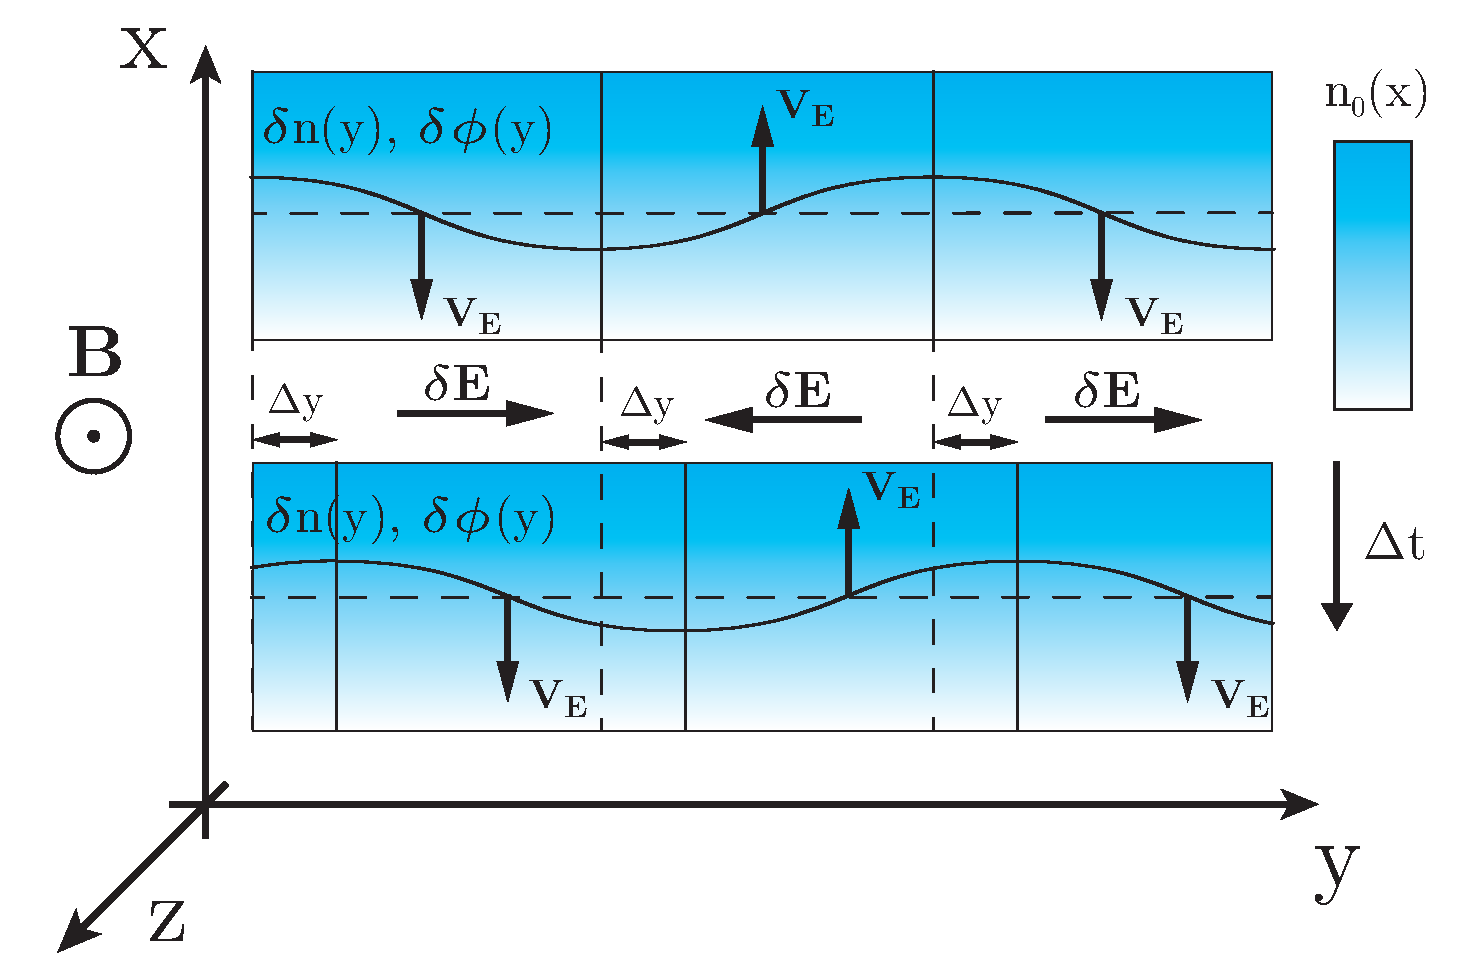
\includegraphics[width=.8\textwidth]{images/drift_wave_diagram.pdf}
    \caption{Propagation of drift-waves through an inhomogeneous plasma, with the background density $n_0(x)$ is shown in blue. Perturbed density $\delta n$ and electrostatic potential $\delta \phi$ fluctuations are considered to be sinusoidal in the $y$ direction. Perturbations in the $z$ direction are not shown for simplicity. The resulting $\mathbf E \times \mathbf B$ velocity, $\mathbf v_E$, is shown to drive an oscillation of the wave to the right, in the $y$ direction, by convecting plasma with higher density to the right of the peak of $\delta n$, and plasma with lower density to the left of the peak.}
    \label{fig:dwfig}
\end{figure}

We now analyze the DW mechanism in the presence of adiabatic electrons.
%
In this case, \cref{eq:adiabaticelectronsreally} shows that the electrostatic potential $\delta \phi$ follows the density perturbations $\delta n$, with a zero phase-shift (see \cref{fig:dwfig}).
%
The electrostatic potential, in turn, creates an electric field $\delta E_{ky} = - i k_\perp \delta \phi_k$ which, according to \cref{eq:dw3}, results in an $\mathbf E \times \mathbf B$ drift in the $x$ direction, i.e., $\mathbf u_{\perp i} = {i k_\perp \delta\phi_k}/B\mathbf e_x$.
%
As shown in \cref{fig:dwfig}, this drift has a maximum at $\delta n=0$ and vanishes when $\delta n$ is at its maximum or minimum.
%
Therefore, the $\mathbf E \times \mathbf B$ velocity and density fluctuations are 90º out of phase.
%
The motion of the plasma along the $x$ direction, driven by the $\mathbf E \times \mathbf B$ velocity, leads to the propagation of the perturbed density to the right, along the $y$ direction, giving rise to the drift-wave.

We note that for finite $R$, a phase-shift is introduced between the electron density and electrostatic potential, resulting in a net transport of particles.
%
In order to accurately describe particle transport in magnetized plasma systems at arbitrary collisionalities, we derive in the next section a moment-hierarchy formalism for DW.

\section{Moment-Hierarchy Model}
\label{sec:momhierarchymodeldw}

While in the EPW case of \cref{ch:epw}, the unmagnetized electron kinetic equation was considered, here we consider the effect of a constant magnetic field and both electron and ion distribution functions are evolved.
%
Under the drift approximation (see \cref{sec:ordering}), the framework to properly treat DW at arbitrary collisionalities is provided by the drift-kinetic equation
%
\begin{equation}
    \frac{\partial F_a}{\partial t} +  \left(v_\parallel \mathbf b + \mathbf v_{E}\right) \cdot \nabla F_a-\nabla_\parallel \phi \frac{q_a}{\sigma_a^2} \frac{\partial F_a}{\partial v_\parallel}= \sum_b \left<C_{ab}\right>,
    \label{eq:dk}
\end{equation}

\noindent where $F_a=F_a(\mathbf R, v_\parallel, \mu, t)$ is the guiding-center distribution function of the species $a$ ($a=e,i$ for electrons and ions, respectively), which depends on the guiding-center coordinate $\mathbf R$, the component of the velocity parallel to the magnetic field $v_\parallel$, the first adiabatic invariant $\mu = m_a v_\perp^2/2 B$ with $m_a$ the mass of the species $a$ and $B$ the modulus of the magnetic field $\mathbf B$, and time $t$ \citep{Hazeltine2003}.
%
The charge $q_a$, the electrostatic potential $\phi$, the parallel and perpendicular scale lengths, $v_\parallel$, and $t$, are normalized to the elementary charge $e$, $T_{e0}/e$, $L_n$, $\rho_s=c_s / \Omega_i$, $c_s=\sqrt{T_{e0}/m_i}$,  $c_s/L_n$ respectively, with $T_{e0}$ a reference temperature, $L_n$ the background density gradient length, and $\Omega_i = e B / m_i$. In addition,  $\mathbf v_E = (L_n/\rho_s) \mathbf b \times \nabla \phi   $ is the dimensionless $\mathbf E \times \mathbf B$ velocity, $\sigma_a = \sqrt{m_a/m_i}$, $\left<C_{ab}\right>=\int_0^{2\pi} d\theta C_{ab}/(2\pi)$ is the gyroaverage operator with $\theta$ the gyroangle, and the Coulomb collision operator is given by \cref{eq:coulombop}.
%
In this chapter, we define $\nu_{ab}$ to be the characteristic collision frequency between species $a$ and $b$ normalized to $c_s/L_n$.
%
The drift-kinetic equation in \cref{eq:dk} corresponds to the one in \cref{eq:boltzmannGC1} when $\mathbf B$ is assumed constant and higher order $(1/\Omega_a)d \mathbf U/dt$ are neglected.
%
The drift-kinetic equation is coupled to Poisson's equation, \cref{eq:poissonfin2}, which with a constant magnetic field, in the quasineutral and cold-ion limit yields
%
\begin{equation}
    \sum_a q_aN_{a}\left(1+\sigma_a^2{\nabla_\perp^2 \phi}{}\right)=0.
\label{eq:quasineutraldw}
\end{equation}
%
In \cref{eq:quasineutraldw}, we define $N_a = \int F_a dv_\parallel d \mu d\theta B/(m_a N_{0})$.

Similarly to \cref{ch:epw}, we linearize \cref{eq:dk} by expressing $F_a = F_{aM}(1 + \delta f_{ka})$ with $\delta f_{ka}\ll 1$ and $F_{aM}$ an isotropic Maxwellian equilibrium distribution function of constant temperature $T_{a0}$ and of density $N_{0}$ that varies perpendicularly to the magnetic field on the $L_n$ scale.
%
This yields

\begin{equation}
\begin{split}
    (\gamma+i k_\parallel v_\parallel)\delta f_{ka} = i\left(k_\perp - q_a k_\parallel v_\parallel \right)\delta\phi_k+\frac{\sum_b \left< C_{ab} \right>}{F_{aM}},
\end{split}
\label{eq:dklinear}
\end{equation}
%
\noindent where $C_{ab}$ is the linearized version of the collision operator in \cref{eq:caa}, $\gamma$ is the growth rate, $k_\parallel$ is the wave-number parallel to $\mathbf B$, and $k_\perp$ is the wave-number along the direction perpendicular to both $\mathbf B$ and the direction of $\nabla N_0$. 
%
As for the EPW case, in this work, we solve \cref{eq:dklinear} at arbitrary collisionality by expanding the distribution function into an orthogonal Hermite-Laguerre polynomial basis, \cref{eq:gyrof}, which for $T_{\parallel a}=T_{\perp a}=T_a$ in normalized units reads
%
\begin{equation}
    f_{a 1} = \sum_{p,j} \frac{N_a^{pj}}{\sqrt{2^p p!}}H_p\left(\frac{v_\parallel \sigma_a}{\sqrt{2 \tau_a}}\right)L_j\left(\frac{\mu B}{T_{a0}}\right),
\end{equation}
%
with $H_p(x)$ the physicists' Hermite polynomials, $L_j$ the Laguerre polynomials, and $\tau_a=T_{a0}/T_{e0}$.
%
By projecting \cref{eq:dklinear} into a Hermite-Laguerre basis, a moment-hierarchy for the evolution of the coefficients of the expansion of $\delta f_{ka}$, $N_{a}^{pj}$, is obtained

\begin{align}
    \gamma N_a^{pj} &= -i k_\parallel \frac{\sqrt{ \tau_a}}{\sigma_a}\left(\sqrt{{p+1}{}}N_a^{p+1 j}+\sqrt{{p}}N_a^{p-1 j}\right)+i\delta\phi_k \left(k_\perp \delta_{p,0}-\frac{q_a k_\parallel}{\sqrt{\tau_a}\sigma_a}\delta_{p,1}\right) \delta_{j,0}+\sum_b C_{ab}^{pj},
\label{eq:dwmomenthierarchy}
\end{align}
%
with $C_{ab}^{pj}=\int \left< C_{ab} \right> H_p L_j dv_\parallel d\mu 2\pi c_s B/(N_0 m_a \sqrt{2^p p!})$ the projection of the Coulomb collision operator $C_{ab}$ onto a Hermite-Laguerre basis.
%
Similarly to \cref{ch:epw}, the Hermite-Laguerre moments of the linearized collision operator $C_{ab}^{pj}$ are obtained by leveraging the work
in \citep{Ji2006}, where $C_{ab}$ is projected onto a tensorial Hermite and associated Laguerre basis, $\mathbf p^{lk}=\mathbf P^{l}(\mathbf c)L_k^{l+1/2}(c^2)$.
%
This yields the gyroaveraged collision operator moments $C^{pj}=\sum_b C_{ab}^{pj}$ in \cref{eq:cabpj}.
%
In addition, we note that, by neglecting ion dynamics and the perpendicular wavevector $k_\perp$ in \cref{eq:dwmomenthierarchy}, we retrieve the EPW moment-hierarchy in \cref{ch:epw}.

A closed form solution for the DW moment-hierarchy can be given in the collisionless case $C_{ab}=0$ by dividing the Boltzmann equation, \cref{eq:dklinear}, by the resonant $\gamma+i k_\parallel v_\parallel$ factor, multiplying by the Hermite-Laguerre polynomial basis functions, and integrating over velocity space, yielding
%
\begin{align}
    {N_a^{pj}}&=\left(-\frac{q_a \xi_a}{\tau_a}+\frac{\sigma_a k_\perp}{k_\parallel\sqrt{\tau_a}}\right)\frac{(-1)^p}{\sqrt{2^p p!}}Z^{(p)}\left(\xi_a\right) \delta\phi_k \delta_{j,0}-\frac{q_a}{\tau_a} \delta\phi_k\delta_{p,0}\delta_{j,0},
\label{eq:npjepw1}
\end{align}
%
where $Z^{(p)}(\xi_a)$ is the $p$th derivative of the plasma dispersion function $Z(\xi_a)=Z^{(0)}(\xi_a)$, defined by $Z^{(p)}(\xi_a)={(-1)^p}\int_{-\infty}^{\infty}{H_p(x)e^{-x^2}}/(x-\xi_a)dx/{\sqrt{\pi}}$
%
\noindent and $\xi_a = \omega \sigma_a/(k_\parallel \sqrt{2\tau_a})$.
%
Equation (\ref{eq:npjepw1}) generalizes the Hermite spectrum obtained for electron-plasma waves, \cref{eq:npjepw}, and extends Hammet-Perkins-like collisionless closures obtained for $N_a^{30}$ and $N_a^{40}$ \citep{Hammett1992a} to a moment $N_a^{pj}$ of arbitrary order in a form ready to be used.

%
The Chapman-Enskog procedure with truncation of the moment-hierarchy in \cref{eq:dwmomenthierarchy} at $p=3$ and $j=1$ can be used in the high collisionality limit, $k_\parallel \lambda_{mfp}\ll 1$.
%
Neglecting sound wave coupling and assuming cold ions, this yields the continuity equation
%
\begin{equation}
    \gamma N=-i( k_\parallel V - k_\perp \delta\phi_k),
\label{eq:contani1}
\end{equation}
%
with $N=N_e^{00}$ the electron density normalized to $N_0$, $V= N_e^{10}/\sigma_e$ the electron parallel fluid velocity normalized to $c_s$, the electron temperature equation
%
\begin{equation}
    \gamma T=- i k_\parallel c_V V- \frac{k_\parallel^2}{\nu} (\chi_{\parallel} T+ 0.12 \Delta T),
\label{eq:tempaniiso}
\end{equation}
%
where $T=(\sqrt{2} N_e^{20}-2 N_e^{01})/3$ is the electron temperature normalized to $T_{e0}$, $\Delta T = \sqrt{2} N_e^{20}+N_e^{01}$ the temperature anisotropy normalized to $T_{e0}$, and $\nu$ the Spitzer resistivity normalized to $c_s/L_n$, the vorticity equation
%
\begin{equation}
    k_\perp^2\gamma\delta\phi_k =i k_\parallel V,
\label{eq:contani}
\end{equation}
%
Ohm's law
%
\begin{equation}
    \sigma_e^2 \gamma V=i k_\parallel(\delta\phi_k-N - c_T T - 0.90 \Delta T) - \nu V,
\label{eq:ohmani}
\end{equation}
%
and temperature anisotropy variation
%
\begin{equation}
    \gamma \Delta T = -12.02 \frac{\nu}{\sigma_e^2} \Delta T - 2.71 i k_{\parallel} V-\frac{k_\parallel^2}{\nu}(0.55 T + 0.52 \Delta T).
\label{eq:tempani}
\end{equation}
%
In \cref{eq:tempaniiso,eq:ohmani}, we have defined the coefficients $(c_T,c_V,\chi_{\parallel})=(1.26,1.88,0.46)$.
%
When temperature anisotropy is neglected (i.e., $\Delta T=0$), the following dispersion relation is obtained
%
\begin{equation}
\begin{split}
    &\sigma_e^2 \gamma^3 + \nu \gamma^2 + \frac{1+ k_\perp^2}{k_\perp^2}k_\parallel^2 \gamma-\frac{i k_\parallel^2}{k_\perp}+\frac{c_V c_T k_\parallel^2 \nu \gamma^2}{\nu \gamma+\chi_{\parallel}{k_\parallel^2}}=0,
\end{split}
\label{eq:drfluid}
\end{equation}
%
which reduces to the drift-reduced Braginskii dispersion relation that has similar coefficients $(c_{V},c_{T},\chi_{\parallel})=(1.14,1.71,1.07)$ \citep{Zeiler1997} (we have checked that the values of the coefficients $(c_T,c_V,\chi_{\parallel})$ approach those computed by Braginskii as the order of the closure is increased).
%
We also note that for resistivity driven DW ($\nu>\gamma m_e/m_i$) the peak growth rate,  $\gamma \simeq 0.12$, is found at $k_\perp \simeq 1.19$ and $k_\parallel = 1.49 \sqrt{\nu}$.
%
If the resistivity $\nu$ in \cref{eq:drfluid} is tuned to values lower than the ones allowed by the fluid approximation ($\nu<\gamma m_e/m_i$) an electron-inertia driven DW is obtained with a peak growth rate $\gamma \simeq 0.29$ at $k_\perp \simeq 1.00$ and $k_\parallel \simeq 0.48 \sqrt{m_e/m_i}$.

%% DWScan Coulomb parameter space

\begin{figure*}
    \centering
    \includegraphics[width=0.99\textwidth]{images/DW_Scan.pdf}
    \caption{Growth rate of the DW instability obtained from the moment-hierarchy, \cref{eq:dwmomenthierarchy}, as a function of $(k_\parallel, k_\perp)$ and, from left to right, $\nu_{ei} =0.05, 1, 10$, and $500$, in the cold-ion limit with $\sigma_e=0.023$.}
    \label{fig:dwscan}
\end{figure*}

%
At intermediate collisionality, the moment-hierarchy equation, \cref{eq:dwmomenthierarchy}, together with Poisson equation have to be solved numerically.
%
In this case, a criterion to truncate the moment expansion at a suitable order $p=P$ and $j=J$ can be derived by following  \citet{Schekochihin2016} where the Lenard-Bernstein operator case was considered.
%
To derive the truncation criterion, we introduce the Fourier harmonics $g_{pj}=i^p \text{sgn}(k_\parallel)^p N_a^{pj}$, and insert them in the moment-hierarchy equation, \cref{eq:dwmomenthierarchy}, noting that at sufficiently high index $p$, $g_p$ can be considered continuous and differentiable in $p$, and therefore $g_{p\pm 1} \simeq g_p \pm \partial_p g_p$.
%
By keeping only the terms proportional to $N_a^{pj}$ in the sum in \cref{eq:cabpj}, namely approximating $C_{ab}^{pj} \simeq - \nu_{ab} f_{pj} N_a^{pj}$ and effectively underestimating the collisional damping contribution of $C_{ab}^{pj}$, we obtain  $g_p\simeq g_0 \exp[-(4 \gamma \sqrt{p} + 2 \int^p f_{p j}p^{-1/2})/p_{ca}]/p^{1/4}$ at the lowest order in $1/p$, with $p_{ca}=4 |k_\parallel|\sqrt{\tau_a}/(\sigma_a \nu_{ai})$.
%
While for the case of the Lenard-Bernstein and Dougherty operators, since $f_{pj} = p+2j$ for large $p$ and $j$, the solution $g_p \simeq g_0 \exp[-4(\gamma \sqrt{p}+p^{3/2}/3)/p_{ca}]/p^{1/4}$ can be obtained analytically, the coefficients $f_{pj}$ for the case of Coulomb collisions are found numerically to follow approximately $f_{pj}\simeq A \sqrt{p}$, with $A \simeq 0.5$.
%
Such estimate yields
%
\begin{equation}
    N_a^{pj}\simeq \frac{N_0(j) i^p \text{sgn}k_\parallel^p}{p^{1/4}}\exp\left[{-\left( {\frac{p}{p_{\gamma a}}}\right)^\frac{1}{2}-2A\frac{p}{p_{c a}}}\right].
    \label{eq:coulpjspectrum}
\end{equation}
%
showing that the moment-hierarchy can be truncated at $P \simeq p_{c a}$ or, if $k_\parallel \lambda_{mfp a} > 2 \gamma^2/A$, at $P \simeq p_{\gamma a} = p_{c a}^2/(16\gamma^2)$ \citep{Zocco2011}.
%
This removes the need of \textit{ad hoc} closures for the moment-hierarchy even at low collisionalities.
%
Regarding the truncation in $j$, since the magnetic field is uniform, no perpendicular phase-mixing in \cref{eq:dwmomenthierarchy} is present, and $j>0$ moments are present due to collisional coupling in $C_{ab}^{pj}$.
%
Therefore, at zero collisionality, the $j>0$ moments vanish [see \cref{eq:npjepw1}].
%
At high collisionality, the Chapman-Enskog closure shows that $j>1$ moments are collisionally damped.
%
At intermediate collisionality, numerical tests show that only moments $j\le 2$ impact the growth rate.
%

%% DWScan Coulomb vs Fluid Study

\begin{figure}
 \centering
 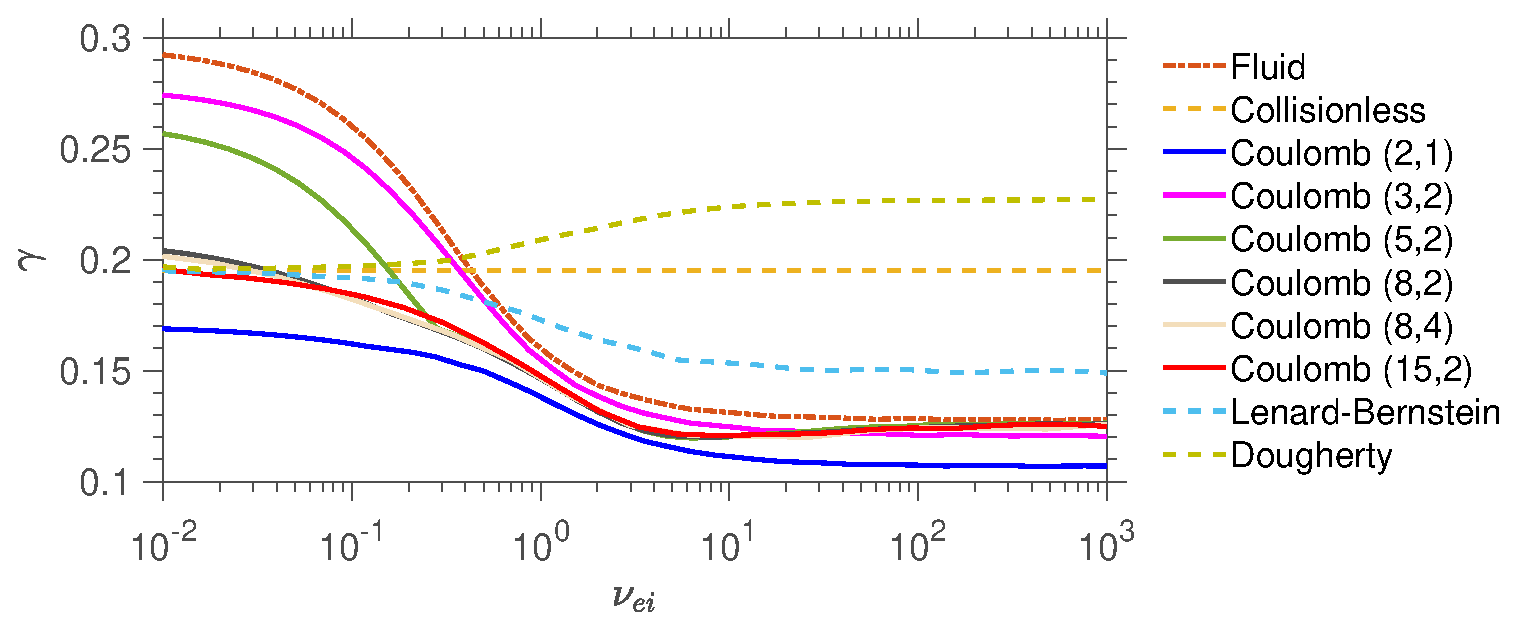
\includegraphics[width=0.99\textwidth]{images/DWscan_gammaPeak_convergence.eps}
 \caption{Comparison of the growth rate $\gamma$ maximized over $k_\parallel$ and $k_\perp$, as a function of collisionality $\nu_{ei}$, between the solution of the drift-reduced Braginskii model, the collisionless model, the linearized moment-hierarchy using a simplified Lenard-Bernstein, Dougherty, and the Coulomb collision operator. For the Coulomb case, truncation at different $(P,J)$ is considered.}
 \label{fig:dwcoulb}
\end{figure}

\section{Numerical Results}
\label{sec:dwnumericalresults}

The numerical solution of the moment-hierarchy, \cref{eq:dwmomenthierarchy}, in the cold-ion limit with $\tau_i=0.01$ and $\sigma_e=0.023$ is shown in \cref{fig:dwscan}, where the maximum growth rate is computed over the $(k_\parallel, k_\perp, \nu_{ei})$ parameter space.
%
The value of $k_\parallel$ at the peak growth rate is seen to increase with $\nu_{ei}$ at large value of the resistivity, as expected from the resistive fluid dispersion relation.
%
For small values of resistivity it converges to $k_\parallel \simeq 0.0074 \simeq 0.32 \sigma_e$, a value close to the fluid predictions for electron-inertia driven DW.
%
The peak growth rate is observed to stay at $k_\perp \simeq 1$ across all values of collisionality, as also expected from the fluid theory.
%
By selecting the $k_\parallel$ and $k_\perp$ that yield the largest growth rate $\gamma$, \cref{fig:dwcoulb} shows a comparison between the peak growth rate resulting from the fluid model, \cref{eq:drfluid}, with the Braginskii values for  $(c_{V},c_{T},\chi_{\parallel})$, the collisionless model, \cref{eq:npjepw1}, and the moment-hierarchy using the Lenard-Bernstein, Dougherty, and the Coulomb collision operator solving for a different number of moments.
%
The linearized moment-hierarchy model approaches the collisionless and the drift-reduced Braginskii model limits, at $\nu_{ei} \ll 1$ and $(\nu_{ei})^{-1} \ll 1$ respectively.
%
Deviations of the peak growth rate of the moment-hierarchy from the drift-reduced Braginskii occur at values of collisionality $\nu_{ei} \lesssim 10$, and from the collisionless limit at $\nu_{ei} \gtrsim 2\times 10^{-2}$.
%
This corresponds to the range $0.1 \lesssim k_\parallel \lambda_{mfp} \lesssim 100$ (at the $k_\parallel$ of the peak growth rate), a range that overlaps with the regime of operation relevant for present and future tokamak machines \citep{Pitts2011}.
%
Deviations of up to $50\%$ with respect to the Lenard-Bernstein and Dougherty operators arise on both the peak growth rate and its corresponding $k_\parallel$ and $k_\perp$.
%
We note that convergence is observed for $P = 15$ and $J=2$ up until $\nu_{ei} \sim 10^{-1}$.
%
The observed value of $P$ is close to the estimate in \cref{eq:coulpjspectrum}, which for $\nu_{ei} = 10^{-1}$ and $k_\parallel \simeq 0.32 \sigma_e$ yields $P \simeq p_{ce} \simeq 13$.
%
We remark that pseudospectral decompositions converge exponentially with the number of modes used.
%
Therefore, with respect to finite-difference methods that display algebraic convergence, the framework proposed here is particularly efficient for numerical implementation.

%% Eigenspectrum Coulomb vs LB Study

\begin{figure}
    \centering
    \includegraphics[width=0.7\textwidth]{images/DW_spectra.pdf}
    \caption{Eigenvalue spectra obtained with the collisionless model, the linearized moment-hierarchy equation using the Coulomb and the Dougherty collision operator {at the wave-number ($k_\parallel$, $k_\perp$) corresponding to the fastest growing mode in the cold-ion limit for $\nu_{ei}=0.4$ and $\sigma_e=0.023$}. The analysis is carried out with $P=15$ and $J=2$.}
    \label{fig:spectra}
\end{figure}

%
We compare in \cref{fig:spectra} the spectra obtained with the collisionless model, and with the Dougherty and the Coulomb collision operators in the moment-hierarchy at $\nu_{ei}=0.4$ for the values of $(k_\parallel, k_\perp)$ that yield the largest $\gamma$.
%
Figure \ref{fig:spectra} shows a clear difference between the eigenmode spectra of the two operators.
%
While modes with finite frequency are related to the damping of electron distribution function, modes at $\omega \ll 1$ are due to strong collisional damping of the cold-ion distribution function.
%
The damping rate of the electron modes decreases with the frequency when the Coulomb collision operator is considered, contrary to the Dougherty case. 
%
This is possibly related to the fact that the collisional drag force decreases with the particle velocity in the Coulomb collision operator and increases in the Dougherty one.
%
We note that the eigenmode spectrum using the Dougherty collision operator in \cref{fig:spectra} is similar to the one obtained in \citet{Bratanov2013} using a Lenard-Bernstein one.

\section{Conclusion}
\label{sec:dwconclusion}

In this chapter, Coulomb collisions are taken into account in the description of magnetized plasma instabilities at arbitrary collisionalities, focusing on the linear properties of the DW instability.
%
The analysis we perform in a relatively simple configuration shows that the corrections introduced by the full Coulomb collision operator with respect to simplified collision operators, presently used in state-of-the-art codes, are qualitatively and quantitatively significant at the relevant collisionality regime of operation of future nuclear fusion devices such as ITER.
%
The results of the present chapter show that the kinetic models introduced in \cref{ch:dk,ch:gk} are a particularly efficient numerical framework to treat Coulomb collisions that can easily be to study other instabilities in magnetized plasmas.
%
Indeed, by projecting onto a Hermite-Laguerre basis the drifts that arise in the Boltzmann equation from possible inhomogeneities of the magnetic field, instabilities such as the ballooning mode, can be described within the framework presented here.
%
Furthermore, we expect that the framework we have introduced in the present thesis can be extended to nonlinear simulations.
